% math0 manuscript template. Build with: latexmk -pdf paper.tex
\documentclass[11pt]{amsart}
\usepackage[margin=1.1in]{geometry}
\usepackage{amsmath,amssymb,amsthm,mathtools}
\usepackage{hyperref}
\usepackage{xcolor}
\usepackage{listings}
\usepackage{newunicodechar}
\usepackage{tikz}

\lstdefinelanguage{lean}{
  keywords={theorem,lemma,def,abbrev,example,fun,by,have,show,from,let,in,if,then,else,match,with,
    namespace,end,open,import,section,variable,instance,structure,where,calc,obtain,intro,exact,
    refine,rcases,rintro,simp,omega,decide,norm_num,linarith,nlinarith,positivity,induction,cases,
    private,noncomputable},
  sensitive=true, comment=[l]{--}, morecomment=[s]{/-}{-/}, string=[b]"}
\lstset{language=lean, basicstyle=\ttfamily\footnotesize, columns=fullflexible, breaklines=true,
  keywordstyle=\color{blue!60!black}\bfseries, commentstyle=\color{gray}, frame=single,
  extendedchars=true, inputencoding=utf8, keepspaces=true,
  literate={ℕ}{{$\mathbb{N}$}}1 {ℤ}{{$\mathbb{Z}$}}1 {∀}{{$\forall$}}1
    {∃}{{$\exists$}}1 {→}{{$\to$}}1 {≤}{{$\le$}}1 {≠}{{$\ne$}}1 {∈}{{$\in$}}1
    {∧}{{$\wedge$}}1 {∨}{{$\vee$}}1 {×}{{$\times$}}1 {α}{{$\alpha$}}1
    {⟨}{{$\langle$}}1 {⟩}{{$\rangle$}}1}
% Unicode commonly found in Lean sources.
\newunicodechar{ℕ}{\ensuremath{\mathbb{N}}}
\newunicodechar{ℤ}{\ensuremath{\mathbb{Z}}}
\newunicodechar{ℚ}{\ensuremath{\mathbb{Q}}}
\newunicodechar{ℝ}{\ensuremath{\mathbb{R}}}
\newunicodechar{ℂ}{\ensuremath{\mathbb{C}}}
\newunicodechar{∀}{\ensuremath{\forall}}
\newunicodechar{∃}{\ensuremath{\exists}}
\newunicodechar{→}{\ensuremath{\to}}
\newunicodechar{←}{\ensuremath{\leftarrow}}
\newunicodechar{↔}{\ensuremath{\leftrightarrow}}
\newunicodechar{↦}{\ensuremath{\mapsto}}
\newunicodechar{¬}{\ensuremath{\neg}}
\newunicodechar{∧}{\ensuremath{\wedge}}
\newunicodechar{∨}{\ensuremath{\vee}}
\newunicodechar{≤}{\ensuremath{\le}}
\newunicodechar{≥}{\ensuremath{\ge}}
\newunicodechar{≠}{\ensuremath{\ne}}
\newunicodechar{∈}{\ensuremath{\in}}
\newunicodechar{∉}{\ensuremath{\notin}}
\newunicodechar{⊆}{\ensuremath{\subseteq}}
\newunicodechar{∩}{\ensuremath{\cap}}
\newunicodechar{∪}{\ensuremath{\cup}}
\newunicodechar{∑}{\ensuremath{\sum}}
\newunicodechar{∏}{\ensuremath{\prod}}
\newunicodechar{⟨}{\ensuremath{\langle}}
\newunicodechar{⟩}{\ensuremath{\rangle}}
\newunicodechar{·}{\ensuremath{\cdot}}
\newunicodechar{∘}{\ensuremath{\circ}}
\newunicodechar{⁻}{\ensuremath{^{-}}}
\newunicodechar{¹}{\ensuremath{^{1}}}
\newunicodechar{²}{\ensuremath{^{2}}}
\newunicodechar{₀}{\ensuremath{_{0}}}
\newunicodechar{₁}{\ensuremath{_{1}}}
\newunicodechar{₂}{\ensuremath{_{2}}}
\newunicodechar{α}{\ensuremath{\alpha}}
\newunicodechar{β}{\ensuremath{\beta}}
\newunicodechar{ε}{\ensuremath{\varepsilon}}
\newunicodechar{δ}{\ensuremath{\delta}}
\newunicodechar{π}{\ensuremath{\pi}}
\newunicodechar{σ}{\ensuremath{\sigma}}
\newunicodechar{φ}{\ensuremath{\varphi}}
\newunicodechar{∞}{\ensuremath{\infty}}
\newunicodechar{⌊}{\ensuremath{\lfloor}}
\newunicodechar{⌋}{\ensuremath{\rfloor}}
\newunicodechar{⌈}{\ensuremath{\lceil}}
\newunicodechar{⌉}{\ensuremath{\rceil}}
\newunicodechar{∣}{\ensuremath{\mid}}
\newunicodechar{≡}{\ensuremath{\equiv}}
\newunicodechar{×}{\ensuremath{\times}}
\newunicodechar{⧸}{\ensuremath{/}}
\newunicodechar{‖}{\ensuremath{\|}}
\newunicodechar{√}{\ensuremath{\surd}}
\newunicodechar{∅}{\ensuremath{\emptyset}}
\newunicodechar{⦃}{\ensuremath{\{\!|}}
\newunicodechar{⦄}{\ensuremath{|\!\}}}
\newunicodechar{𝓝}{\ensuremath{\mathcal{N}}}
\newunicodechar{≫}{\ensuremath{\gg}}
\newunicodechar{≪}{\ensuremath{\ll}}

\theoremstyle{plain}
\newtheorem{theorem}{Theorem}
\newtheorem{lemma}[theorem]{Lemma}
\newtheorem{proposition}[theorem]{Proposition}
\newtheorem{corollary}[theorem]{Corollary}
\theoremstyle{definition}
\newtheorem{definition}[theorem]{Definition}
\newtheorem{remark}[theorem]{Remark}

\emergencystretch=3em
% Lean identifiers in running text (breakable at dots and underscores).
\expandafter\def\expandafter\UrlBreaks\expandafter{\UrlBreaks\do\_\do\.}
\DeclareUrlCommand\decl{\urlstyle{tt}}
\newcommand{\N}{\mathbb{N}}
\newcommand{\Z}{\mathbb{Z}}
\newcommand{\C}{\mathcal{C}}
\newcommand{\G}{\mathcal{G}}
\newcommand{\Stab}{\operatorname{Stab}}
\newcommand{\cls}{\operatorname{N}}

\title[Inequivalent cells of $(6k+5)$-iamonds]{The least number of inequivalent cells in a polyiamond with $6k+5$ cells}
\author{math0}
\address{Produced by Claude (an AI model developed by Anthropic) in the math0 project}
\date{October 20, 2026}

\begin{document}
\begin{abstract}
OEIS A369366 lists the least number $a(n)$ of inequivalent cells in a polyiamond with $n$ cells, two cells being equivalent when a symmetry of the polyiamond maps one to the other. We prove Peter Exley's conjecture that $a(6k+5)=3(k+1)$ for all $k\ge0$; the entry reports it as observed only for $k=0,1,2$. The lower bound is a coordinate version of the argument in Exley's own comment, and the bound is attained by the straight row of $6k+5$ triangles. Both halves are elementary; we classify the note as a new result, whose new content is the matching construction and a complete proof. The proof is verified in Lean~4 against a statement that math0 formalized from the OEIS entry, checked in the kernel against the first eight listed terms, reviewed for fidelity and frozen before the proof attempt.
\end{abstract}
\maketitle

\section{Introduction}

A \emph{polyiamond} with $n$ cells is an edge-connected set of $n$ triangles of the regular triangular tiling of the plane, holes allowed (A000577 \cite{A000577}). Two cells of a polyiamond $P$ are \emph{equivalent} if some isometry of the plane maps $P$ onto itself and one cell to the other. The OEIS sequence A369366 \cite{A369366}, contributed by Pontus von Brömssen on January~22, 2024, is the least number $a(n)$ of inequivalent cells in a polyiamond with $n$ cells, with data $1,1,2,2,3,1,3,3,3,3,6,2,4,4,4,4,9,2,5,6$ for $n=1,\dots,20$ ($a(18)$ by John Mason, 2024; $a(19),a(20)$ by Peter Exley, 2026). Related entries are A369365 \cite{A369365} (free rooted polyiamonds), A369367 \cite{A369367} (the number of polyiamonds attaining $a(n)$), and the analogues for polyominoes, polyhexes and polycubes, A367758 \cite{A367758}, A369363 and A376798. In a comment of April~7, 2026, Exley wrote (verbatim):
\begin{quote}\raggedright\small
\texttt{For n = 6k+5, no rotational symmetry is possible (n = 2 mod 3 blocks 3-fold rotation; n odd blocks 180-degree rotation), giving |G\_max| = 2 and a(6k+5) >= ceiling(n/2) = 3(k+1).} [\dots]\\[2pt]
\texttt{Conjecture: a(6k+5) = 3(k+1) for all k >= 0. Observed for k = 0, 1, 2 (n = 5, 11, 17). The next test case is a(23), predicted to be 12.}
\end{quote}

\subsection*{Prior work}
Exley's comment thus contains the lower bound $a(6k+5)\ge3(k+1)$ with a sketch of its proof. The math0 referees read the entry at revision \#14 (April~14, 2026) and its edit history: it gives no construction attaining the bound for general $k$. The entry links a repository of Exley's code \cite{Exley}, which the referees could not inspect (HTTP 404). The cross-referenced entries A369365, A369367, A369363, A369364, A367758, A367759, A373637, A376798 and A376799 contain no proof for polyiamonds; the only related proof is Mason and von Brömssen's proof of a closed formula for the polyomino analogue A367758 \cite{MvB}, a different problem on the square lattice. Searches of arXiv and the general web found no resolution of the conjecture, and it is not among the statements of formal-conjectures \cite{FC} (commit \texttt{c77fdd4}).

\subsection*{Contribution}
We prove the conjecture (Theorem~\ref{thm:main}). The lower bound (Proposition~\ref{prop:lower}) proves the bound of Exley's comment in integer coordinates, for every set of $6k+5$ cells, connected or not. For the upper bound we observe that the straight row of $2m+1$ triangles has a mirror symmetry exchanging its $j$-th and $(2m-j)$-th cells, so it has at most $m+1$ classes (Proposition~\ref{prop:upper}). Both steps are elementary. The proof is checked in Lean~4 (Section~\ref{sec:lean}). In particular $a(23)=12$, as Exley predicted.

\section{Statement}\label{sec:statement}

We use the integer coordinates of the formal statement. For $x\in\Z^3$ put $\sigma(x)=x_1+x_2+x_3$ and $\|x\|_1=|x_1|+|x_2|+|x_3|$.

\begin{definition}\label{def:main}
(1) The \emph{cells} are the points of $\C=\{x\in\Z^3:\sigma(x)\in\{0,1\}\}$; cells $x,y$ are \emph{adjacent} if $\|x-y\|_1=1$. A \emph{polyiamond with $n$ cells} is a set $P\subseteq\C$ with $|P|=n$ in which any two cells are joined by a chain of cells of $P$, consecutive cells being adjacent.

(2) Let $\Pi$ be the group of the six coordinate permutations of $\Z^3$. A \emph{grid symmetry} is a triple $g=(\pi,\varepsilon,t)$ with $\pi\in\Pi$, $\varepsilon\in\{1,-1\}$, $t\in\Z^3$, and $\sigma(t)=0$ if $\varepsilon=1$, $\sigma(t)=1$ if $\varepsilon=-1$; it acts by $g(x)=\varepsilon\,\pi(x)+t$. Let $\G$ be the set of grid symmetries.

(3) For finite $P\subseteq\Z^3$ let $\Stab(P)=\{g\in\G: g(P)=P\}$. Write $c\sim_P d$ if $g(c)=d$ for some $g\in\Stab(P)$. Let $\cls(P)$ be the number of classes of $\sim_P$ on $P$, and $a(n)=\min\{\cls(P): P\text{ a polyiamond with $n$ cells}\}$.
\end{definition}

\begin{theorem}[Exley's conjecture]\label{thm:main}
For every integer $k\ge0$, $a(6k+5)=3(k+1)$.
\end{theorem}

\subsection*{Encoding}
The tiling is cut by three families of parallel lines. A triangle is labelled by the indices $(x_1,x_2,x_3)$ of the strips of the three families that contain it, shifted so that $\sigma(x)=0$ for one orientation of triangles and $\sigma(x)=1$ for the other. Each point of $\C$ labels exactly one triangle, and two triangles share an edge exactly when they are separated by one grid line and lie in the same strips of the other two families, that is, when $\|x-y\|_1=1$. The coordinate permutations exchange the line families, $x\mapsto -x+(\text{const})$ is a half-turn, and the translations of the tiling are the $t\in\Z^3$ with $\sigma(t)=0$; so $\G$ is the symmetry group $p6m$ of the tiling. The entry's equivalence uses all symmetries of the polyiamond, reflections included (``free'' rooted polyiamonds in A369365). This gives the same classes: an isometry of the plane mapping a polyiamond onto itself maps its corners, which are vertices of the tiling, to corners and edge directions at a corner to edge directions, so it is a symmetry of the tiling.

\subsection*{Lean formalization}
The statement was formalized by math0 in \path{lean/Math0/Statements/OEIS/A369366.lean}, reviewed for fidelity, and frozen before any proof attempt (SHA-256 hash beginning \texttt{3bce9518}). Its definitions and the statement read as follows, verbatim except that comments, docstrings, the proof of \decl{a_data} and all lemmas and auxiliary definitions between \decl{a} and \decl{a_data} are omitted:
\begin{lstlisting}
namespace Math0.Statements.A369366
abbrev Pt := ℤ × ℤ × ℤ
def sumC (x : Pt) : ℤ := x.1 + x.2.1 + x.2.2
def IsCell (x : Pt) : Prop := sumC x = 0 ∨ sumC x = 1
def Adj (x y : Pt) : Prop := |y.1 - x.1| + |y.2.1 - x.2.1| + |y.2.2 - x.2.2| = 1
def perm {α : Type} (s : Fin 6) (x : α × α × α) : α × α × α :=
  match s.val with
  | 0 => (x.1, x.2.1, x.2.2)
  | 1 => (x.1, x.2.2, x.2.1)
  | 2 => (x.2.1, x.1, x.2.2)
  | 3 => (x.2.1, x.2.2, x.1)
  | 4 => (x.2.2, x.1, x.2.1)
  | _ => (x.2.2, x.2.1, x.1)
def lin (s : Fin 6) (neg : Bool) (x : Pt) : Pt := if neg then -perm s x else perm s x
def tReq (neg : Bool) : ℤ := if neg then 1 else 0
structure Isom where
  s : Fin 6
  neg : Bool
  t : Pt
  ht : sumC t = tReq neg
def Isom.app (g : Isom) (x : Pt) : Pt := lin g.s g.neg x + g.t
def Step (P : Finset Pt) (u v : Pt) : Prop := u ∈ P ∧ v ∈ P ∧ Adj u v
def IsConnected (P : Finset Pt) : Prop :=
  ∀ x ∈ P, ∀ y ∈ P, Relation.ReflTransGen (Step P) x y
def IsPolyiamond (n : ℕ) (P : Finset Pt) : Prop :=
  P.card = n ∧ (∀ x ∈ P, IsCell x) ∧ IsConnected P
def Equivalent (P : Finset Pt) (c d : Pt) : Prop :=
  ∃ g : Isom, P.image g.app = P ∧ g.app c = d
open Classical in
noncomputable def cls (P : Finset Pt) (c : Pt) : Finset Pt := P.filter (Equivalent P c)
noncomputable def numClasses (P : Finset Pt) : ℕ := (P.image (cls P)).card
noncomputable def a (n : ℕ) : ℕ :=
  sInf {m | ∃ P : Finset Pt, IsPolyiamond n P ∧ numClasses P = m}
theorem a_data : (List.range 8).map (fun i => a (i + 1)) = [1, 1, 2, 2, 3, 1, 3, 3]
def statement : Prop := ∀ k : ℕ, a (6 * k + 5) = 3 * (k + 1)
end Math0.Statements.A369366
\end{lstlisting}
Here \decl{Isom} is $\G$ (\texttt{neg = true} means $\varepsilon=-1$), \decl{Equivalent} is $\sim_P$ (proved to be an equivalence relation in the file), \texttt{cls P c} is the class of $c$, and \texttt{numClasses P} $=\cls(P)$ counts the distinct classes. \texttt{a n} is an infimum in $\N$ over a set that is nonempty for $n\ge1$ (it contains $\cls(T_n)$ of Section~\ref{sec:upper}), so the convention $\inf\emptyset=0$ plays no role. The statement is the conjecture for all $k\ge0$, with no further hypotheses.

The theorem \decl{a_data} checks the listed terms $a(1),\dots,a(8)$. As \decl{a} is not computable, the file defines an enumeration \decl{aComp} of polyiamonds up to grid symmetry and proves $a(n)=$ \texttt{aComp n} for $n\ge1$ (\decl{a_eq_aComp}, using only soundness and completeness of the enumeration and the invariance of \decl{numClasses} under $\G$); the values are then computed by \texttt{decide +kernel}, in about a minute. Later terms are not checked in the kernel, since each further term roughly triples the cost. The fidelity reviewer recomputed in Python, on the same encoding, the numbers of free polyiamonds with $n\le13$ cells (matching A000577) and $a(1),\dots,a(13)$ (matching the data); a referee recomputed $a(1),\dots,a(12)$ with a geometric model of the tiling.

\section{Proof}\label{sec:proof}

We follow the Lean proof; Lean names are given in brackets. The statement file proves the facts about $\G$ that we use. Each $\pi\in\Pi$ is additive and preserves $\sigma$ and $\|\cdot\|_1$. Each $g\in\G$ is a bijection of $\Z^3$ that maps $\C$ to $\C$ and preserves adjacency. $\G$ is closed under composition and inverses:
\[
  (\pi,\varepsilon,t)\circ(\pi',\varepsilon',t')=(\pi\pi',\varepsilon\varepsilon',\varepsilon\pi(t')+t),\qquad (\pi,\varepsilon,t)^{-1}=(\pi^{-1},\varepsilon,-\varepsilon\pi^{-1}(t)).
\]
Hence so is $\Stab(P)$. For finite $P$, $g(P)\subseteq P$ already gives $g(P)=P$. Let $\Pi^+=\{\mathrm{id},\rho,\rho^2\}$, where $\rho(x_1,x_2,x_3)=(x_2,x_3,x_1)$, be the even permutations (indices $0,3,4$ of \decl{perm}) and $\Pi^-$ the three transpositions (indices $1,2,5$). Geometrically, the symmetries with $\varepsilon=1$ preserve the orientation of every cell (translations, $\pm120^\circ$ rotations, and reflections and glide reflections with $\pi\in\Pi^-$). Those with $\varepsilon=-1$ exchange the two orientations (half-turns, $\pm60^\circ$ rotations, and the remaining reflections and glide reflections). The proofs below do not use this dictionary.

\subsection{Lower bound}

\begin{lemma}[\decl{neg_eq_false}]\label{lem:neg}
Let $P\subseteq\Z^3$ be finite with $|P|$ odd, and $g=(\pi,\varepsilon,t)\in\Stab(P)$. Then $\varepsilon=1$.
\end{lemma}

\begin{proof}
If $\varepsilon=-1$, then $\sigma(g(x))=-\sigma(\pi x)+\sigma(t)=1-\sigma(x)$ for all $x$. As $g$ permutes $P$, $S=\sum_{x\in P}\sigma(x)$ satisfies $S=\sum_{x\in P}\sigma(g(x))=\sum_{x\in P}(1-\sigma(x))=|P|-S$, so $|P|=2S$ is even.
\end{proof}

\begin{lemma}[\decl{rot3_cube}, \decl{rot3_fix}]\label{lem:rot3}
Let $g=(\pi,1,t)\in\G$ with $\pi\in\{\rho,\rho^2\}$. Then (1) $g(g(g(x)))=x$ for all $x\in\Z^3$, and (2) $g$ fixes at most one cell.
\end{lemma}

\begin{proof}
(1) As $\pi$ is additive, $g^3(x)=\pi^3(x)+\pi^2(t)+\pi(t)+t$. Here $\pi^3=\mathrm{id}$, and since $\pi$ permutes the coordinates cyclically, each coordinate of $\pi^2(t)+\pi(t)+t$ is $\sigma(t)=0$.
(2) If $x,y\in\C$ are fixed, then $\pi(x-y)=(g(x)-t)-(g(y)-t)=x-y$. A vector fixed by a cyclic shift has equal coordinates, so $x-y=(d,d,d)$ and $3d=\sigma(x)-\sigma(y)\in\{-1,0,1\}$. Hence $d=0$. (In Lean: a case split on $\pi$, then \texttt{omega}.)
\end{proof}

\begin{lemma}[\decl{no_rot3}]\label{lem:norot3}
If $P\subseteq\C$ is finite with $|P|\equiv2\pmod3$, then $\Stab(P)$ contains no $(\pi,1,t)$ with $\pi\in\{\rho,\rho^2\}$.
\end{lemma}

\begin{proof}
Such a $g$ restricts to $f\colon P\to P$ with $f^3=\mathrm{id}_P$ (Lemma~\ref{lem:rot3}(1)). If a self-map $f$ of a finite set satisfies $f^{p^r}=\mathrm{id}$ with $p$ prime, then $f$ is a bijection whose orbits have size $1$ or a positive power of $p$, so the size of the set is congruent modulo $p$ to the number of fixed points (Mathlib's \decl{Equiv.Perm.card_fixedPoints_modEq}, here with $p=3$, $r=1$). By Lemma~\ref{lem:rot3}(2), $f$ has at most one fixed point, so $|P|\equiv0$ or $1\pmod3$, a contradiction.
\end{proof}

\begin{lemma}[\decl{rot_trivial}]\label{lem:rot}
Let $P\subseteq\C$ be finite with $|P|\equiv5\pmod 6$ and $g=(\pi,\varepsilon,t)\in\Stab(P)$ with $\pi\in\Pi^+$. Then $g$ is the identity of $\Z^3$.
\end{lemma}

\begin{proof}
$\varepsilon=1$ by Lemma~\ref{lem:neg}, and $\pi\notin\{\rho,\rho^2\}$ by Lemma~\ref{lem:norot3}, as $|P|\equiv2\pmod3$. So $g(x)=x+t$, and since $g$ permutes $P$, $\sum_{x\in P}x=\sum_{x\in P}g(x)=\sum_{x\in P}x+|P|\,t$. Hence $t=0$, as $P\neq\emptyset$. (In Lean this is the statement file's centroid lemma \decl{t_eq_of_sym}: $t=(s-\varepsilon\pi(s))/|P|$, componentwise, for $g\in\Stab(P)$ and $s=\sum_{x\in P}x$.)
\end{proof}

\begin{lemma}[\decl{three}, \decl{card_cls_le}]\label{lem:three}
Let $P\subseteq\C$ be finite with $|P|\equiv5\pmod6$. (1) If $c\sim_P d$ and $c\sim_P e$, then $d=c$, $e=c$ or $d=e$. (2) Every class of $\sim_P$ has at most two elements.
\end{lemma}

\begin{proof}
(1) Let $d=g(c)$, $e=h(c)$ with $g,h\in\Stab(P)$, with permutation parts $\pi_g,\pi_h$. If $\pi_g\in\Pi^+$, then $d=c$ by Lemma~\ref{lem:rot}; likewise $e=c$ if $\pi_h\in\Pi^+$. Otherwise $\pi_g,\pi_h\in\Pi^-$, and $k=h\circ g^{-1}\in\Stab(P)$ has the even permutation part $\pi_h\pi_g^{-1}$ (\decl{mulTab_inv_even}, nine cases checked by \texttt{decide}). By Lemma~\ref{lem:rot}, $k=\mathrm{id}$, so $e=h(c)=k(g(c))=d$.
(2) Three distinct cells $x,y,z$ of one class satisfy $x\sim_P y$ and $x\sim_P z$, and (1) with $c=x$ gives a contradiction.
\end{proof}

\begin{proposition}[\decl{lower}]\label{prop:lower}
If $P\subseteq\C$ is finite with $|P|\equiv5\pmod6$, then $|P|\le2\,\cls(P)$. In particular $\cls(P)\ge3k+3$ if $|P|=6k+5$.
\end{proposition}

\begin{proof}
The $\cls(P)$ classes partition $P$ and have at most two elements each (Lemma~\ref{lem:three}). In Lean this is \decl{Finset.card_le_mul_card_image} for $c\mapsto$ \texttt{cls P c}. If $|P|=6k+5$, then $2\cls(P)\ge6k+5$, so $\cls(P)\ge3k+3$.
\end{proof}

Compared with Exley's sketch: Lemma~\ref{lem:neg} excludes all symmetries that exchange the two cell orientations, half-turns included. Lemmas~\ref{lem:rot3} and~\ref{lem:norot3} exclude the $120^\circ$ rotations, and Lemma~\ref{lem:three} replaces the claim $|G_{\max}|=2$.

\subsection{Upper bound}\label{sec:upper}

For $j\in\N$ let $s_j=(\lceil j/2\rceil,-\lfloor j/2\rfloor,0)$ (\decl{stripCell}) and $T_n=\{s_j:0\le j<n\}$ (\decl{strip}). All cells of $T_n$ have third coordinate $0$, so they lie in one row between two adjacent parallel grid lines: $T_n$ is the straight row of $n$ triangles of alternating orientation. For odd $n=2m+1\ge3$ it is an isosceles trapezoid with parallel sides of lengths $m$ and $m+1$ (Figure~\ref{fig:strip}).

\begin{figure}[ht]
\centering
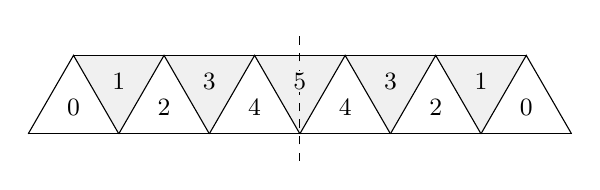
\begin{tikzpicture}[scale=1.15]
\pgfmathsetmacro{\h}{0.8660254}
\foreach \i in {0,...,4} {
  \fill[gray!12] (\i+0.5,\h) -- (\i+1.5,\h) -- (\i+1,0) -- cycle;
}
\draw[dashed] (3,-0.3) -- (3,\h+0.3);
\draw (0,0) -- (6,0) (0.5,\h) -- (5.5,\h);
\foreach \i in {0,...,5} {
  \draw (\i,0) -- (\i+0.5,\h) -- (\i+1,0);
}
\foreach \j in {0,...,10} {
  \pgfmathtruncatemacro{\c}{min(\j,10-\j)}
  \ifodd\j
    \node[fill=gray!12,inner sep=1pt] at ({(\j+1)/2},{2*\h/3}) {\small $\c$};
  \else
    \node[fill=white,inner sep=1pt] at ({(\j+1)/2},{\h/3}) {\small $\c$};
  \fi
}
\end{tikzpicture}
\caption{The row $T_{11}$ ($k=1$, $m=5$); cells with $\sigma=1$ are shaded. The cell $s_j$ carries the number $\min(j,10-j)$. The mirror $\mu$ of Lemma~\ref{lem:mirror} (dashed axis) exchanges cells with equal numbers, so $T_{11}$ has at most $6=3(k+1)$ classes, and by Proposition~\ref{prop:lower} exactly $6$.}
\label{fig:strip}
\end{figure}

\begin{lemma}[\decl{stripCell_adj}, \decl{strip_isPolyiamond}]\label{lem:strip}
The map $j\mapsto s_j$ is injective, each $s_j$ is a cell adjacent to $s_{j+1}$, and $T_n$ is a polyiamond with $n$ cells.
\end{lemma}

\begin{proof}
The first coordinate of $s_j$ minus the second is $\lceil j/2\rceil+\lfloor j/2\rfloor=j$, and $\sigma(s_j)=\lceil j/2\rceil-\lfloor j/2\rfloor\in\{0,1\}$. For $j=2i$, $s_j=(i,-i,0)$ and $s_{j+1}=(i+1,-i,0)$; for $j=2i+1$, $s_j=(i+1,-i,0)$ and $s_{j+1}=(i+1,-i-1,0)$. So $\|s_{j+1}-s_j\|_1=1$. Hence $|T_n|=n$, $T_n\subseteq\C$, and for $i\le j<n$ the chain $s_i,s_{i+1},\dots,s_j$ in $T_n$ joins $s_i$ to $s_j$; reversed, it joins $s_j$ to $s_i$.
\end{proof}

\begin{lemma}[\decl{mirror_app}, \decl{equivalent_mirror}]\label{lem:mirror}
For $m\in\N$ let $\mu=(\tau,1,(m,-m,0))$ with $\tau(x_1,x_2,x_3)=(x_2,x_1,x_3)$, i.e.\ $\mu(x)=(x_2+m,x_1-m,x_3)$. Then $\mu\in\G$, $\mu(s_j)=s_{2m-j}$ for $0\le j\le 2m$, $\mu\in\Stab(T_{2m+1})$, and $s_j\sim_{T_{2m+1}}s_{2m-j}$.
\end{lemma}

\begin{proof}
$\sigma(m,-m,0)=0$, so $\mu\in\G$. For $0\le j\le2m$, $\mu(s_j)=(m-\lfloor j/2\rfloor,\ \lceil j/2\rceil-m,\ 0)=s_{2m-j}$, because $\lceil(2m-j)/2\rceil=m-\lfloor j/2\rfloor$ and $\lfloor(2m-j)/2\rfloor=m-\lceil j/2\rceil$. So $\mu(T_{2m+1})\subseteq T_{2m+1}$, hence $\mu(T_{2m+1})=T_{2m+1}$.
\end{proof}

\begin{proposition}[\decl{upper}]\label{prop:upper}
For every $m\in\N$, $\cls(T_{2m+1})\le m+1$.
\end{proposition}

\begin{proof}
Each class is that of some $s_j$, $0\le j\le 2m$. If $j>m$, then $s_j\sim s_{2m-j}$ with $2m-j<m$ (Lemma~\ref{lem:mirror}). So every class is that of one of $s_0,\dots,s_m$.
\end{proof}

\begin{proof}[Proof of Theorem~\ref{thm:main}]
Let $n=6k+5$ and $A=\{\cls(P):P\text{ a polyiamond with $n$ cells}\}$, so $a(n)=\inf A$. With $m=3k+2$, $2m+1=n$, so $\cls(T_n)\in A$ by Lemma~\ref{lem:strip} and $\cls(T_n)\le3k+3$ by Proposition~\ref{prop:upper}; hence $a(n)\le3k+3$ (\decl{Nat.sInf_le}). Every element of the nonempty set $A$ is at least $3k+3$ by Proposition~\ref{prop:lower}, so $a(n)\ge3k+3$ (\decl{le_csInf}).
\end{proof}

\begin{remark}
Proposition~\ref{prop:upper} gives $a(2m+1)\le m+1$ for all $m$, but for odd $n\not\equiv5\pmod6$ this need not be attained, e.g.\ $a(7)=3<4$. The minimizers are not unique: by A369367 there are $2$, $27$ and $523$ of them for $n=5,11,17$. Our argument says nothing about these counts.
\end{remark}

\section{Machine verification}\label{sec:lean}

The proof is in \path{lean/Math0/Frontier/OEIS/A369366.lean} in the math0 repository, \url{https://github.com/Foundation-0/math0}. It imports the frozen statement file and the audit commands in \path{lean/Math0/Audit.lean}. The main declaration is the theorem \decl{Math0.Frontier.A369366.result}, of type \decl{Math0.Statements.A369366.statement}. All other declarations in the file are private: the lemmas and definitions named in Section~\ref{sec:proof}, the helpers \decl{fin6_cases}, \decl{stripCell_injective}, \decl{stripCell_isCell}, \decl{stripCell_mem}, \decl{rtg_symm}, \decl{mirror}, \decl{cls_eq}, and three \texttt{rfl} lemmas unfolding \decl{perm}. The proof involves no finite computation beyond the nine-case \texttt{decide} and \texttt{fin\_cases} on $\mathrm{Fin}\,6$; the kernel computation \decl{a_data} of the statement file is not used. Neither file uses \texttt{sorry}, \texttt{native\_decide} or a \texttt{maxHeartbeats} option.

\subsection*{Audit}
The file ends with the command \texttt{\#math0\_settles} applied to \decl{Math0.Frontier.A369366.result} and \decl{Math0.Statements.A369366.statement}. This command, defined in \path{lean/Math0/Audit.lean} for statements that math0 formalizes itself, fails unless (1) \decl{statement} is a definition of type \texttt{Prop} without universe parameters; (2) \decl{statement} and \decl{result} depend on no axioms other than \decl{propext}, \decl{Classical.choice} and \decl{Quot.sound}, which rejects \decl{sorryAx}, the axioms \decl{Lean.ofReduceBool} and \decl{Lean.trustCompiler} behind \texttt{native\_decide}, and custom axioms; and (3) the type of \decl{result} is syntactically the statement or its negation, up to metadata annotations and with no unfolding. On this file it reports:
\begin{lstlisting}
math0 audit: 'Math0.Statements.A369366.statement' depends on axioms [Classical.choice, Quot.sound, propext]
math0 audit: 'Math0.Frontier.A369366.result' depends on axioms [Classical.choice, Quot.sound, propext]
math0 statement check: 'Math0.Frontier.A369366.result' proves 'Math0.Statements.A369366.statement'
\end{lstlisting}

\subsection*{Toolchain and reproduction}
We use Lean~4 \cite{Lean4} \texttt{v4.33.1} and Mathlib \cite{Mathlib} \texttt{v4.33.1}, pinned in \path{lean/}. The repository also pins formal-conjectures \cite{FC} at commit \texttt{c77fdd4}, which this result does not use. Running \path{scripts/verify.sh} from the repository root fetches the Mathlib build cache, builds all math0 results with \texttt{lake build} (re-running every audit), checks that the pinned \texttt{formal\_conjectures} and \texttt{mathlib} checkouts are unmodified, and reports the number of statement checks that passed. For this result alone, run, in \path{lean/}, \texttt{lake build Math0.Statements.OEIS.A369366} (including the kernel check of \decl{a_data}: about a minute and 4~GB of memory) and then \texttt{lake env lean Math0/Frontier/OEIS/A369366.lean}, which takes about 15 seconds on our machine, mostly loading Mathlib.

\begin{thebibliography}{99}

\bibitem{Exley}
P.~Exley, \emph{Solver code, verifiers, and data}, GitHub repository \url{https://github.com/pexley-math/oeis-A369366}, linked from \cite{A369366}; not accessible to the referees (HTTP 404) in October 2026.

\bibitem{FC}
M.~Firsching, P.~Lezeau, S.~Mercuri, M.~Z. Horv\'ath, Y.~Dillies, C.~S\"onne, E.~Wieser, F.~Zhang, T.~Hubert, B.~Ag\"uera y Arcas, and P.~Kohli, \emph{Formal Conjectures: An Open and Evolving Benchmark for Verified Discovery in Mathematics}, arXiv:2605.13171, 2026. Repository: \url{https://github.com/google-deepmind/formal-conjectures}.

\bibitem{MvB}
J.~Mason and P.~von Brömssen, \emph{Proof of formula}, attachment to OEIS A367758 (formula added October~8, 2024), \url{https://oeis.org/A367758/a367758.pdf}.

\bibitem{Mathlib}
The mathlib Community, \emph{The Lean mathematical library}, in: Proceedings of the 9th ACM SIGPLAN International Conference on Certified Programs and Proofs (CPP 2020), ACM, 2020, 367--381.

\bibitem{Lean4}
L.~de Moura and S.~Ullrich, \emph{The Lean 4 theorem prover and programming language}, in: Automated Deduction -- CADE 28, Lecture Notes in Comput. Sci. \textbf{12699}, Springer, 2021, 625--635.

\bibitem{A000577}
The OEIS Foundation Inc., \url{https://oeis.org/A000577} (number of polyiamonds with $n$ cells, turning over and holes allowed).

\bibitem{A367758}
The OEIS Foundation Inc., \url{https://oeis.org/A367758}, entry by P.~von Brömssen (2023): least number of inequivalent cells in a polyomino with $n$ cells.

\bibitem{A369365}
The OEIS Foundation Inc., \url{https://oeis.org/A369365}, entry by P.~von Brömssen (2024): number of free rooted polyiamonds with $n$ cells.

\bibitem{A369366}
The OEIS Foundation Inc., \url{https://oeis.org/A369366}, entry by P.~von Brömssen (2024), with comments and the conjecture by P.~Exley (April~7, 2026); revision \#14.

\bibitem{A369367}
The OEIS Foundation Inc., \url{https://oeis.org/A369367}, entry by P.~von Brömssen (2024), comments by P.~Exley (2026): number of free polyiamonds with $n$ cells attaining A369366$(n)$.

\end{thebibliography}

\end{document}
